\documentclass[10pt]{article}

% amsmath package, useful for mathematical formulas
\usepackage{amsmath}
% amssymb package, useful for mathematical symbols
\usepackage{amssymb}

% graphicx package, useful for including eps and pdf graphics
% include graphics with the command \includegraphics
\usepackage{graphicx}
\usepackage{epstopdf}
\graphicspath{ {./figures/} }

% cite package, to clean up citations in the main text. Do not remove.
\usepackage{cite}
\usepackage{color}
\usepackage{soul}
\usepackage{longtable}
\usepackage{pdfpages}
\usepackage{color}

% Text layout
\topmargin 0.0cm
\oddsidemargin 0.5cm
\evensidemargin 0.5cm
\textwidth 16cm 
\textheight 21cm

% Bold the 'Figure #' in the caption and separate it with a period
% Captions will be left justified
\usepackage[labelfont=bf,labelsep=period,justification=raggedright]{caption}


\bibliographystyle{plain}

% Remove brackets from numbering in List of References
\makeatletter
\renewcommand{\@biblabel}[1]{\quad#1.}
\makeatother


% Leave date blank
\date{}

\pagestyle{myheadings}
%% ** EDIT HERE **

\newcommand{\beginsupplement}{%
        \setcounter{table}{0}
        \renewcommand{\thetable}{S\arabic{table}}%
        \setcounter{figure}{0}
        \renewcommand{\thefigure}{S\arabic{figure}}%
     }


%% END MACROS SECTION

\begin{document}

\begin{flushleft}
{\Large
\textbf{The Metabolic Landscape of Tumors}
}
% Insert Author names, affiliations and corresponding author email.
\\
E Reznik, A Luna, BA Aksoy, C Sander, others less worthy
\\
$^1$ Computational Biology Center, Sloan-Kettering Institute, New York NY

$^\ast$ E-mail: reznike@mskcc.org
\end{flushleft}

\begin{abstract}
- Assembled 13 studies, 9 cancer types, ~1K samples, benchmark for future meta-analyses?
- Examined intrinsic variation associated with normal--> tumor transformation
- Recurrent metabolic alterations
- Clinical association with metabolites
\end{abstract}

\section{Introduction}
One approach to studying cancer biology is to widely profile the genomes, epigenomes, or proteomes of large cohorts of tumors and benign tissues. This paradigm has proven fruitful for the identification, via statistical recurrence, of molecular alterations evident across many tumor types and likely driving cancer. The result of such efforts by groups like The Cancer Genome Atlas (TCGA) is a detailed census of hallmark mutations, copy number alterations, methylation events, and proteomic changes driving many cancer types.

In contrast, while the deregulation of metabolism is a well-accepted hallmark of cancer, surveys of metabolic alterations in tumors have remained limited in scope. Tumors must grow and divide in the face of stress imposed by indefinite proliferation and augmented by cytotoxic and targeted therapy. To do so, cancer cells modulate the activity of metabolic pathways to supplant ATP production, produce suitable levels of biosynthetic precursors, sustain redox potential and maintain epigentic integrity. As a whole, these metabolic alterations are implemented via changes in the levels of intracellular metabolites, enzymes, and transporters. Restricted by the availability of adequate data, signatures of recurrent metabolic alterations have only been investigated through analysis of changes to the expression of metabolic genes. To our knowledge, no comparable investigation has surveyed changes to the dual of the metabolic transcriptome: the universe of small chemical constituents of the cell known as the metabolome.

At a basic level, we seek to understand whether the abundances of metabolites are dysregulated in a common manner across different cancers. To do so, we will describe an integrative analysis of metabolomic data from eleven studies of nine different tumor types. Where possible, our analysis is supplemented with limited clinical annotation, which enables a first-order analysis of clinical features associated with the progression of tumors. 

To complete such a meta-analysis, we will face some challenges unique to metabolomics data. Unlike genomic sequencing, which frequently covers the full breadth of the exome or genome, metabolomics relies on the targeted identification of a small (on the order of hundreds) library of small molecules. Each individual metabolomic study is likely to profile distinct, partially overlapping assortments of these molecules, and inconsistent use of standard nomenclature (\textit{e.g.} KEGG or CHEBI IDs} makes their alignment across studies challenging. Furthermore, because most metabolomics studies to date have utilized mass spectrometry, metabolite abundances are reported in relative (rather than absolute) units. In the work that follows, we will describe our informatic approach to resolving these issues.


\begin{figure}[ht!]
  \centering
     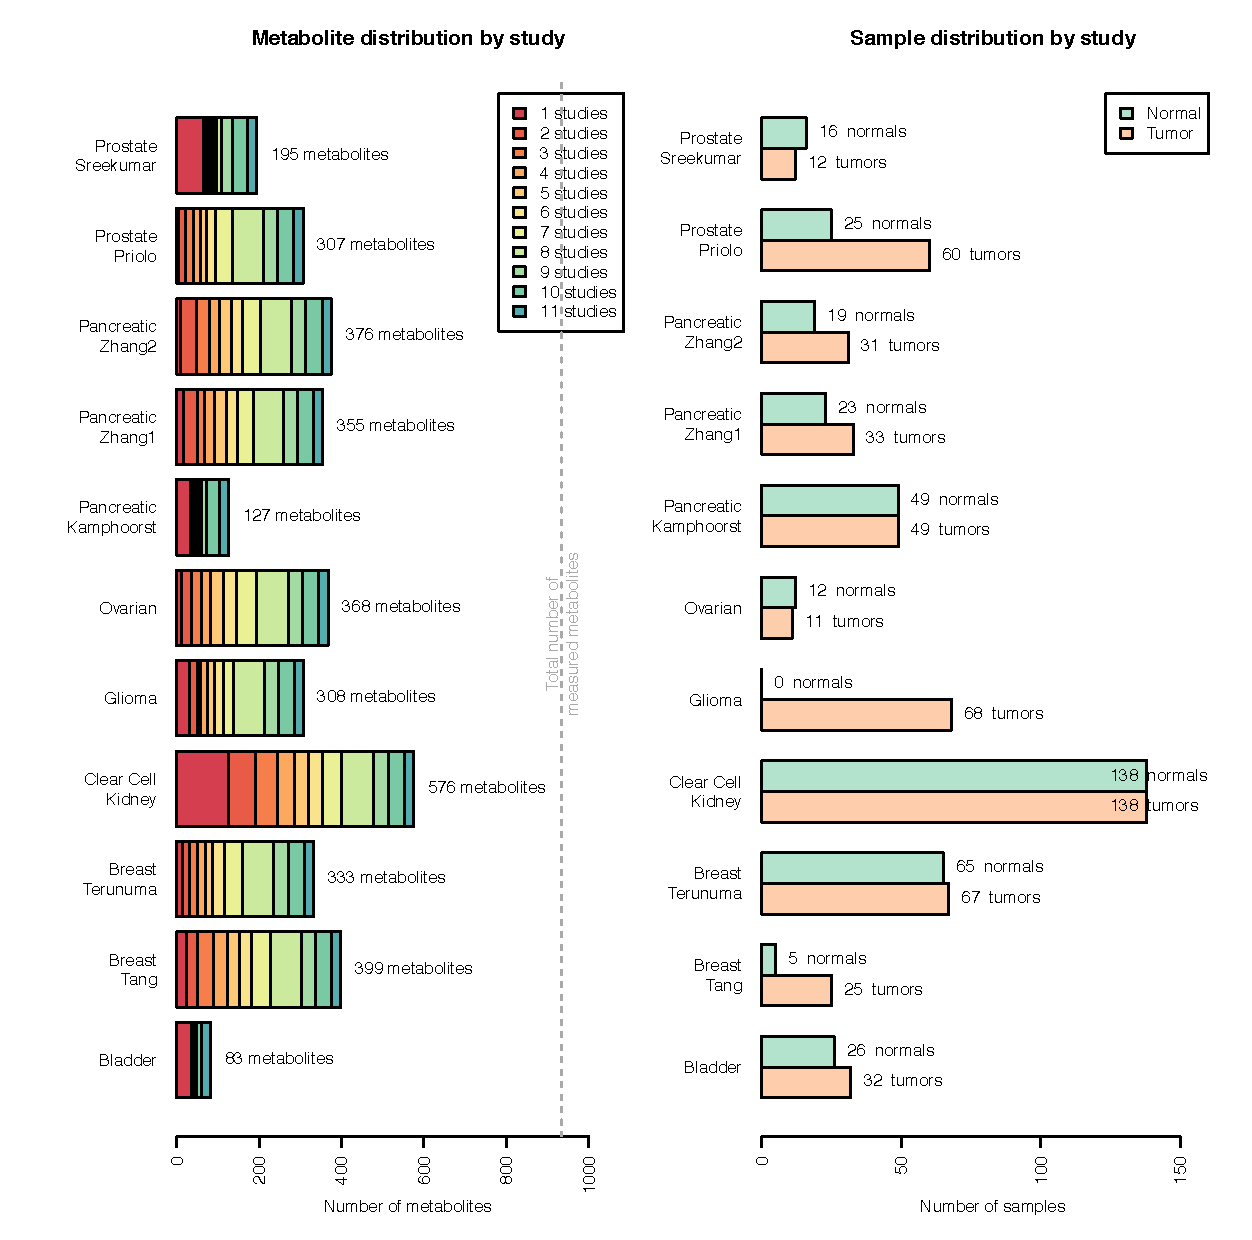
\includegraphics[scale = 0.5]{finalfigures/Figure1.pdf}
  \caption{\textbf{Metabolomics data analyzed in this study.} Data from 11 distinct metabolomics studies, examining 7 cancer types, were aggregated. Due to incomplete coverage of the metabolome, many metabolites were profiled in a small proportion of studies. The number of tumor/normal samples varied from study to study, and all but one study (gliomas) contained normal samples.}
     \label{fig:Fig1}
\end{figure}

\section{Assembly of a Cross-Cancer Compendium of Metabolomics Data}
We obtained published cancer tissue metabolomics data from eleven datasets covering seven distinct cancer types (see Figure \ref{fig:Fig1} and Supplementary Table 1). Data for all studies was collected using mass spectrometry. Three cancer types (breast, prostate, and pancreatic ductal adenocarcionoma \cite{Hirayama2009}) were represented by at least 2 different datasets, enabling us to evaluate the consistency of findings across different studies. In total, our dataset encompasses 935 distinct small molecule compounds across 928 tissue samples. 

To complete a meta-analysis, we implemented a data standardization pipeline (Figure \ref{fig:Fig2}) addressing two independent problems: quantatitative standardization of metabolomic measurements, and bioinformatic alignment of metabolites profiled across many studies (see Methods for detailed description). Data generated from mass spectrometry studies were in general reported as relative quantifications of metabolites (\textit{i.e.} peak intensities), rather than absolute measures of concentration. making direct comparison of the same metabolite across studies infeasible (see Figure \ref{fig:Fig2}). Furthermore, across all studies, a number of metabolites were at sufficiently low abundance so as to fall outside the sensitivity of the measuring instrument, and were often imputed. Making this data amenable to quantitative analysis was essential, because it contained useful information indicating that the concentration of a metabolite was low (compared to samples where the concentration was within the quantifiable limits). To enable a fair comparison of metabolomics data across different studies, we implemented a common data imputation and standardization pipeline.

In addition to data standardization, a bioinformatic challenge to our meta-analysis was the identification of metabolites profiled across multiple studies. Unlike other high-throughput technologies which can measure the abundance of all relevant species in a sample (\textit{e.g.} RNA sequencing), metabolomic profiling samples only a fraction of all compounds in the metabolite. More importantly, metabolites are referred to by different synonymous names (\textit{e.g.} lactate, lactic acid, (S)-2-Hydroxypropanoate, all refer to the same molecule), and are often reported alongside a variety of identifiers (\textit{e.g.} KEGG IDs, HMDB IDs, Pubchem IDs). To address this issue, we searched for synonymous identifiers of each metabolite using the Chemical Translation Service (CITE). These identifers were then used to assemble a meta-dataset of all metabolomics data, ``aligning'' metabolites sharing common identifiers. Manual inspection of the aligned dataset confirmed that our method correctly matched metabolites across different studies. All code for data standardization and alignment is provided at Bitbucket (URL).

\begin{figure}[ht!]
  \centering
     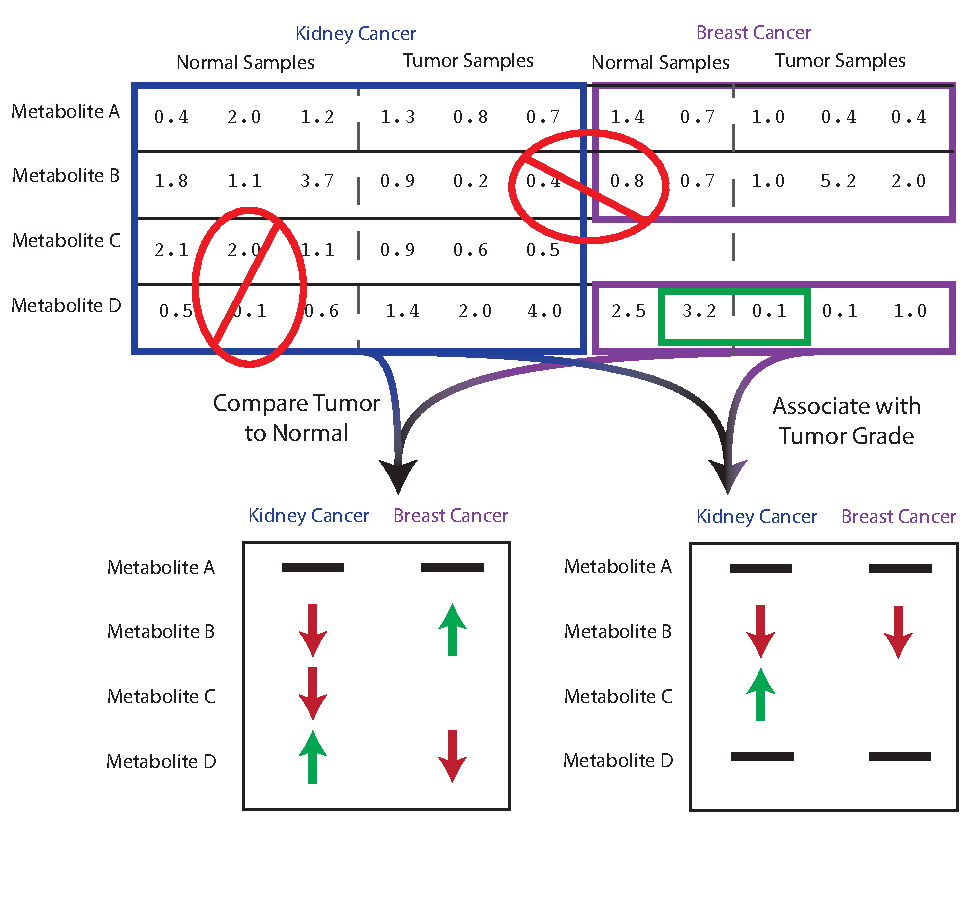
\includegraphics[scale = 0.75]{finalfigures/Figure2_Data.pdf}
  \caption{Metabolomics data aggregated from different studies cannot be directly compared. Typically, for each metabolite, abundance is reported relative to the median of all measurements of a metabolite within a study. Comparisons between different metabolites profiled in the same study is not directly possible (leftmost red box). Furthermore, comparisons between the same metabolite profiled across different studies is not possible	(topmost red box). Throughout our analysis, we will frequently examine the change in abundance of a single metabolite across different subsets of tissue samples (\textit{e.g.} tumor/normal samples) from the same study (green box). }
     \label{fig:Fig2}
\end{figure}

\section{Analysis of Metabolic Variation in Tumors and Normal Tissue}
Large sequencing efforts have revealed the remarkable diversity of mechanisms which can drive the transformation of normal tissue to tumor. In some cases, tumors are characterized by a handful of genetic mutations, while in others, hundreds or thousands of mutations may collude to drive the tumor \cite{Martincorena2015}. In analogy to these studies, we sought to understand whether the differences between tumor/normal tissue varied substantially across different tumor types. 

Therefore, on a study-by-study basis, we examined which metabolites were differentially abundant between tumor and normal samples (Mann-Whitney U test, BH-corrected p-value < 0.05). We found the number of differentially abundant metabolites varied drastically from one cancer type to the next (Figure \ref{fig:Fig3}A). For example, in studies of breast and clear-cell kidney tumors, we found that greater than 40 percent of metabolites showed at least a 2-fold change in abundance, whereas two independent studies of prostate cancer found that fewer than 6 percent of metabolites were differentially abundant. Importantly, because the number of tumor/normal samples were comparable for breast and prostate cancers, the differences in differential abundance were unlikely to be statistical artifacts arising from differences in sample size. 

It is also possible that tumors and normal tissues differ in the inherent variability of metabolite levels, without exhibiting differential abundance. To test this possibility, we estimated the median absolute deviation (MAD), a non-parametric measure of the variability of a collection of measurements. For each metabolite (and separately for each study), the ratio of MAD in tumor and normal samples was calculated. To control for potential sample-size biases, only data with paired tumor and adjacent-normal samples was used. The distribution of MAD ratios for a given cancer type indicates whether metabolite levels were inherently more variable in tumors (distribution shifted to the right of zero) or less variable in tumors (distribution shifted to the left) compared to normal tissue. We observed major differences in variability across tumor types: breast and kidney tumors were significantly more variable than their normal tissue counterparts, while all PDAC tumors were significantly less variable than their normal tissue counterparts. Together with the results above, these results speak to the major differences in metabolic alterations associated with each individual cancer type. 

This analysis also revealed a cancer-type-dependent trend towards unequal proportions of metabolites which increased or decreased between tumor and normal tissues. In both breast cancer studies, we found that nearly all metabolites deemed differentially abundant were at higher levels in tumor tissue, compared to normal tissue. Similar results were reported in the original publications for these two datasets \cite{Terunuma2014,Tang2015}. While similar biases were evident in other studies (\textit{.e.g.} differentially abundant metabolites in pancreatic tumors tended to be at lower concentration in tumors), the effect was particularly striking for breast cancer. Although it is not possible for us to determine with certainty the source of this effect, we speculate it could arise from the disproportionate extent of data imputation for metabolites in normal breast tissue, compared to the extent of imputation in tumor tissue (Figure \ref{fig:SIFig_Imputation}). Because the effect is apparent in both breast cancer studies, it may be possible that metabolites are broadly at higher concentrations in breast tumor compared to benign breast tissue.

\begin{figure}[ht!]
  \centering
     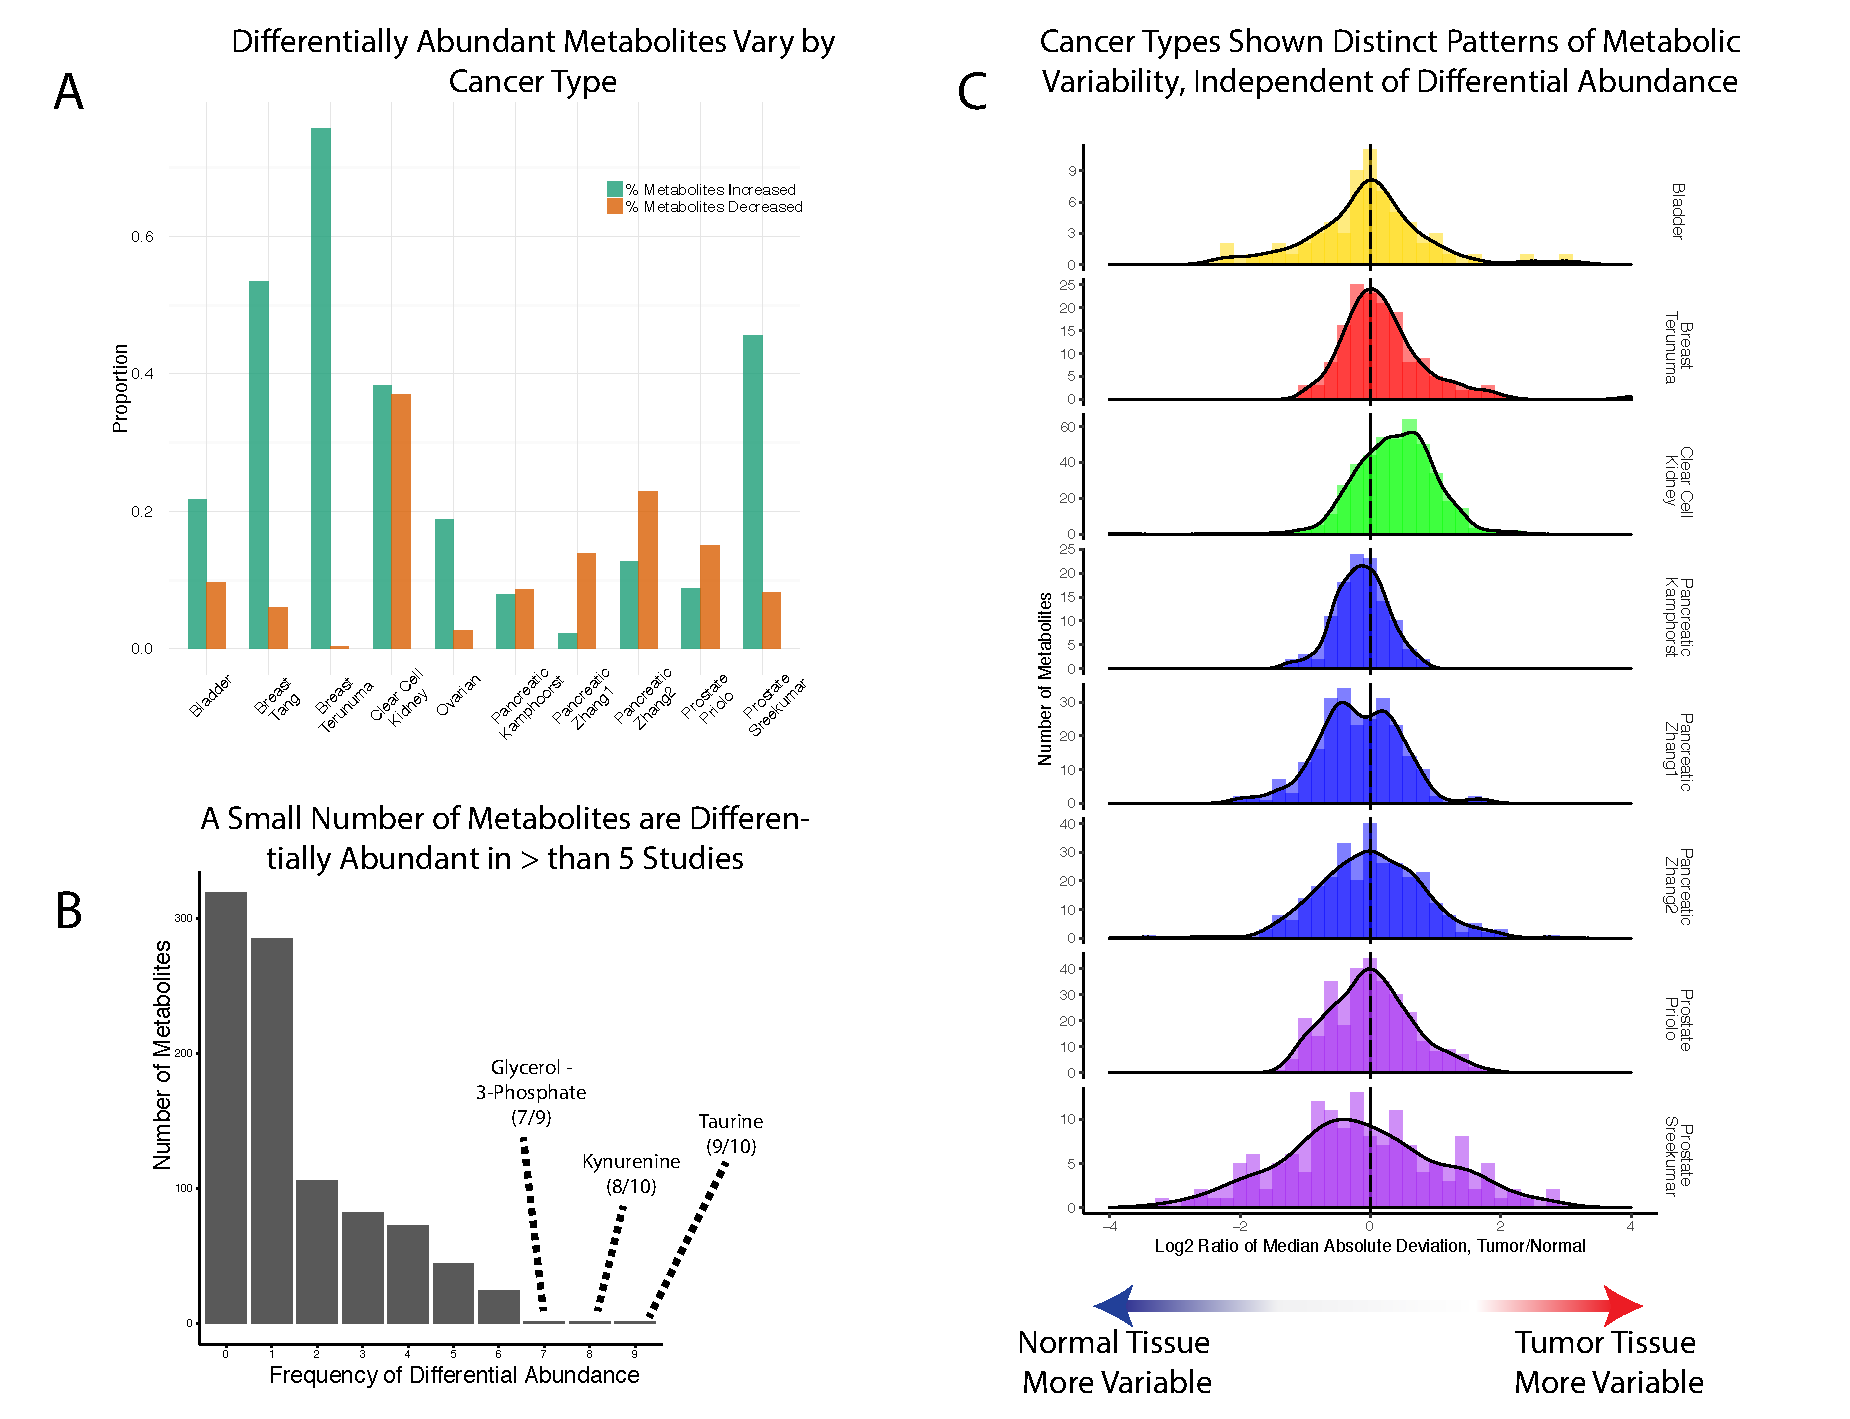
\includegraphics[scale = 0.5]{finalfigures/Figure3.pdf}
  \caption{\textbf{Tumor/Normal Comparison.} (A) Comparison of metabolic alterations in tumors to natural metabolic variation in normal tissue. By comparing the similarity of (1) randomly chosen pairs of tumor/normal tissues, to (2) randomly chosen pairs of normal tissues, we assessed the magnitude of change associated with cancerous transformation. Metabolic alterations in prostate and pancreatic tumors are small when compared with natural metabolic variation in these tissues. (B) The number of differentially abundant metabolites between tumor and normal tissues across each study varies by cancer type. Breast tumors contain the most differentially abundant metabolites, while prostate tumors contain the least. }
     \label{fig:Fig3}
\end{figure}

\section{Common Patterns of Metabolic Alterations Across Cancers}
Cancers share common genetic alterations despite inherent physiological and molecular differences in their tissue of origin. Because of a lack of data, it has not been possible to assess whether metabolic alterations, manifested through shifts in the abundances of metabolites from tumors to normal tissue, are also common across different cancer types. 

By aggregating the results of our differential abundance screen, we identified 30 metabolites differentially abundant in at least 5 studies (Supplementary Table XX). Among these, a single metabolite, taurine, was differentially abundant in eight of the ten studies in which it was measured. \textcolor{red}{Justin: is there something special about taurine that we should mention?}. Drilling deeper, only a handful of metabolites were uniformly elevated in 5 or more studies (with no findings of significant depletion in any tumor type): three acyl-carnitine species (acetyl-,hexonyl-, and butyryl-), beta-alanine, kynurenine, and lactate. Comparatively fewer metabolites showed a tendency towards recurrent depletion in cancers. Only a single metabolite, pelargonate, was depleted in 4 different studies (BRCATang,KIRC, and PDAC), and two other fatty acids (laurate and myristate) were depleted in three different studies. 

Among the metabolites which showed recurrent differential abundance, several have been previously implicated in the development or progression of cancer. Perhaps the best studied example is lactate, the terminal product of the high-flux, energy-producing pathway of glycolysis, and the metabolite originally described by Otto Warburg as elevated in cancerous tissues. Kynurenine, in contrast, is a derivative of tryptophan which is well-known to have immunosuppresive properties when secreted into the extracellular milieu \textcolor{red}{citations!}. Acyl-carnitines are generated by beta-oxidation of fatty acids, and are used to refuel the TCA cycle with acetyl-CoA, and their general elevation in tumors may indicate an increased reliance on fatty acid catabolism in tumors. The depletion of fatty acids in these cancer types may reflect increased $\beta$-oxidation of fatty acids, and be a mirror image of increased levels of acyl-carnitines. 

\textcolor{red}{Work on this, is it even worth mentioning?}Elevated levels of lactate in tumors are likely derived from increased flux through glycolysis, a metabolic feature which has found widespread clinical utility in FDG-PET imaging (CITE). We decided to investigate the elevation of lactate in tumors in greater detail, leveraging a subset of our data for which we had paired instances of tumor and adjacent-normal tissue. To our surprise, We found that 84/347 (24\%) of tumor samples contained lower levels of lactate than their matched normal tissue counterpart. While most studies were enriched for tumors with increased levels of lactate, prostate tumors were the outliers: the majority of prostate tumors showed reduced levels of lactate relative to paired adjacent normal tissue. While reduced tumor lactate levels is not necessarily a surrogate for glycolytic flux, the finding that nearly a quarter of tumors appear to contain lower concentrations of lact

\section{Pathway Analysis}
An alternative way of understanding the broad patterns of metabolic alterations is through analysis of functional pathways into which metabolites may be organized. To make greater sense of which metabolic processes may be recurrently up- or down-regulated in tumors, we aggregated the differential abundance results across KEGG metabolic pathways. For each study, we mapped metabolites onto KEGG pathways, and calculated an aggregate differential abundance score for each pathway (see Methods). We restricted our analysis to pathways for which at least 5 metabolites in the pathway were profiled across 6 or more studies, leaving us with XX total pathways. 

Generally, pathway-level changes in abundances of metabolites were heterogeneous across cancer types, with no single pathway uniformly elevated across all studies. Some pathways, however, did show trends corresponding to frequent elevation/depletion. Pathways associated with sugar metabolism (\textit{e.g.} fructose/mannose metabolism, glycolysis/gluconeogenesis, and amino sugar and nucleotide sugar metabolism) were generally elevated. Many tumor types also showed increases in glutathione metabolism, which produces the cell's primary antioxidant (reduced glutathione, GSH). Interestingly, we found that only a single pathway, fatty acid biosynthesis, showed recurrent recurrent depletion of its constituent metabolites across cancers. 
\begin{figure}[ht!]
  \centering
     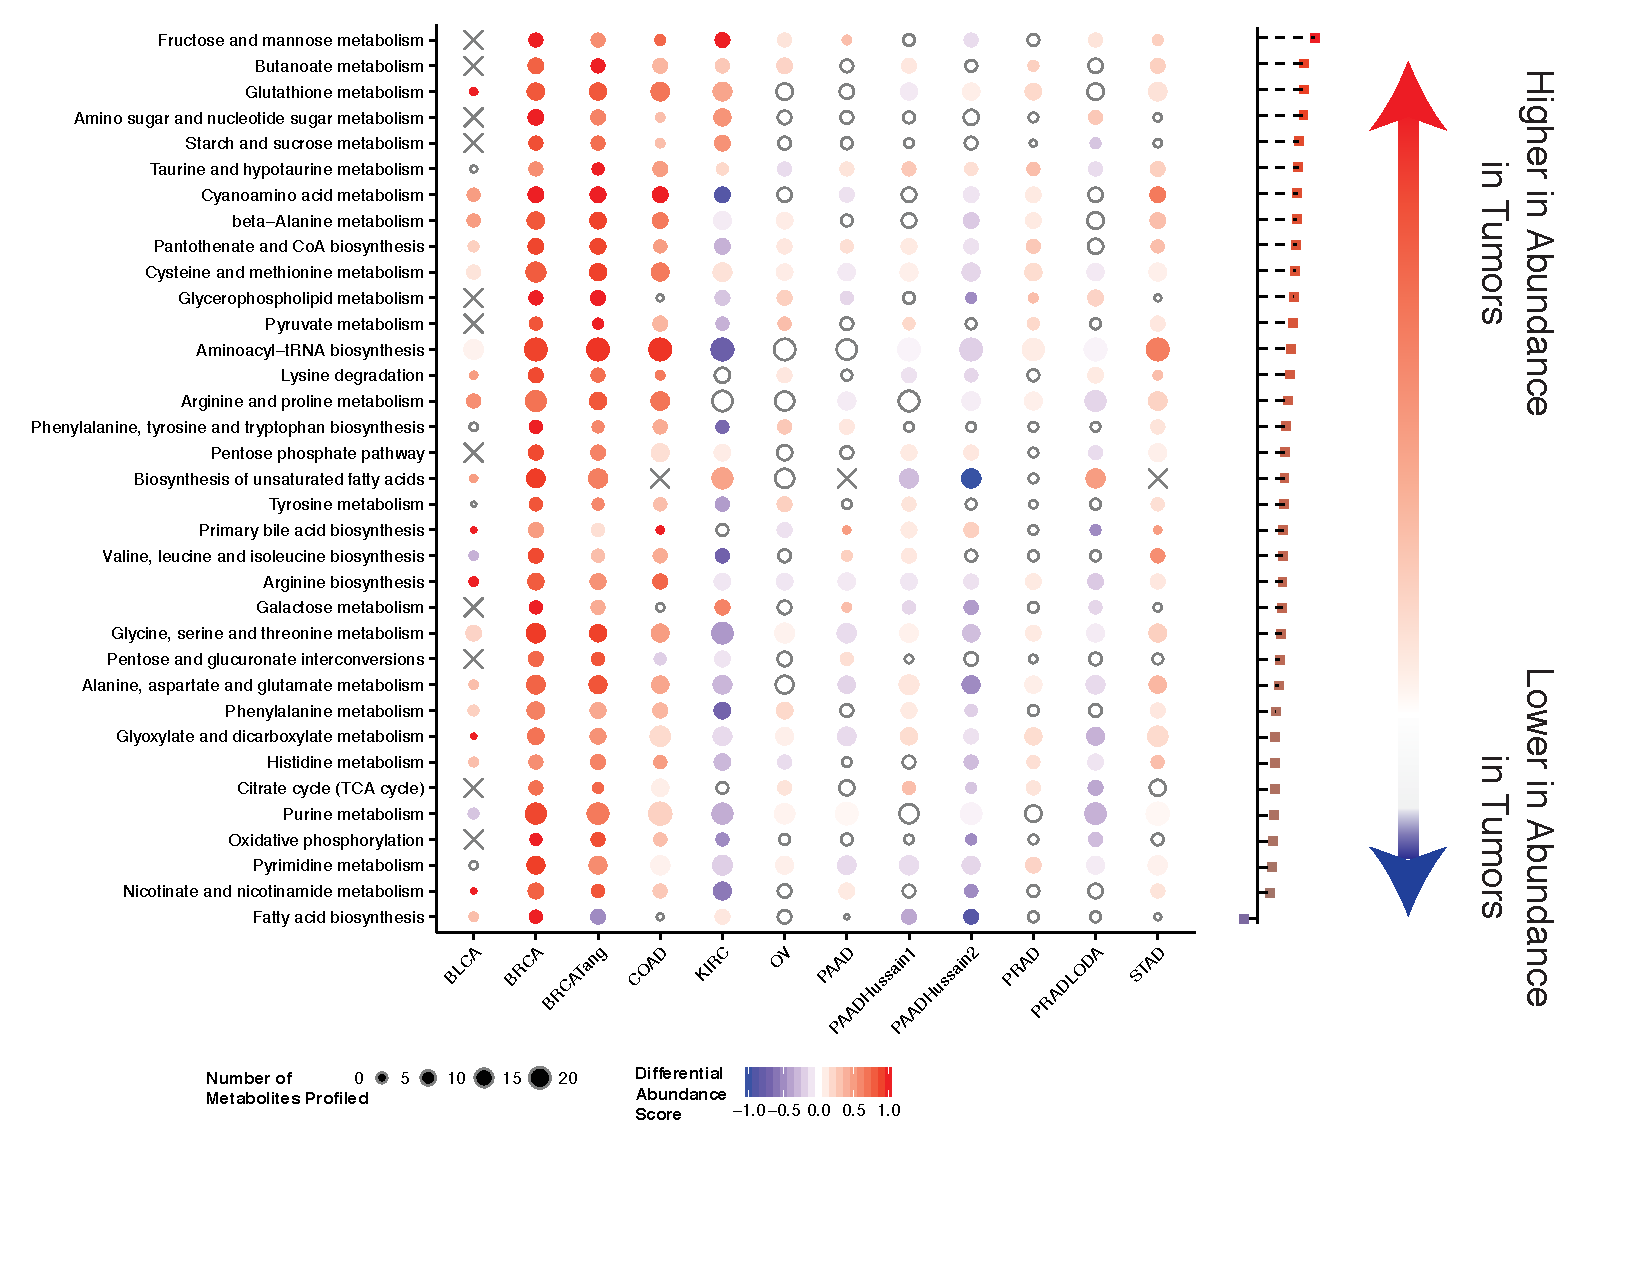
\includegraphics[scale = 0.5]{finalfigures/Figure4.pdf}
  \caption{\textbf{Recurrent metabolic alterations.} (A) Heatmap of metabolites which are differentially abundant across at least 8 different cancer studies. (B) Pathway analysis \textcolor{red}{Write more.}}
     \label{fig:Fig4}
\end{figure}


\section{Metabolic Indicators of Tumor Progression}
Tumors become clinically aggressive by acquiring genetic, physiological, and morphological features that enable them to metastasize.  These features can be distinct from In light of this, we examined our data for metabolic signals associated with progression of tumors to higher grade, \textcolor{red}{is this correct: a histological measure of the extent of abnormal apperance of tumor cells}. Among the eleven cancer studies which we collected in our dataset, five had associated clinical data on tumor grade. We used statistical meta-analysis techniques to identify metabolites which showed consistent changes (\textit{i.e.} consistent increase/decrease in metabolite levels with increasing tumor grade) across several cancer types. Our analyis accounted for the frequency of imputed data (see detailed description in Methods).

In total, we found 140 metabolites whose abundance were significantly correlated to tumor grade, and 60 metabolites with abundances significantly correlated to tumor stage. Filtering these results further to extract metabolites significantly associated with clinical features across many tumor types, we found 14 metabolites associated to tumor grade in at least 3 studies, including several amino acids (asparagine, proline, phenylalanine, leucine), 3 pyrimidines and their derivatives (thymine, uracil, and 5,6-dihydrouracil), and kynurenine. 

Among the most interesting findings was the observation that kynurenine levels were increased in tumors versus normal tissues. Kynurenine is a metabolic byproduct of the degradation of trytophan by two groups of enzymes: tryptophan dioxygenases and indoleamine 2,3-dixoygenases. Binding of kynurenine to aryl hydrocarbon receptors (AHRs) and suppress the activity of T-effector cells, as well as indirectly activating regulatory pro-tumorigenic T cells. Kynurenine was unique in our study because it was found to be elevated in the majority of tissues, and it was also found to be positively correlated to tumor grade in 4 different studies (2 different prostate cancer studies, as well as breast cancers and gliomas). Together, these findings point to a critical role for kynurenine in the metabolism of tumors.

We also considered the possibility that tumor grade may effect the metabolic profile of adjacent-normal tissue. Such an association could arise in several ways; for example, nearby tumor tissue may alter the microenvironment surrounding adjacent-normal tissue (a field effect), or alternatively the physiology of patients with more aggressive tumors may lead to changes in the metabolic features of an entire organ. To evaluate this possibility, we repeated the analysis described above using metabolite abundances from normal tissue samples from patients for which we had clinical information. Surprisingly, we identified 

\begin{figure}[ht!]
  \centering
     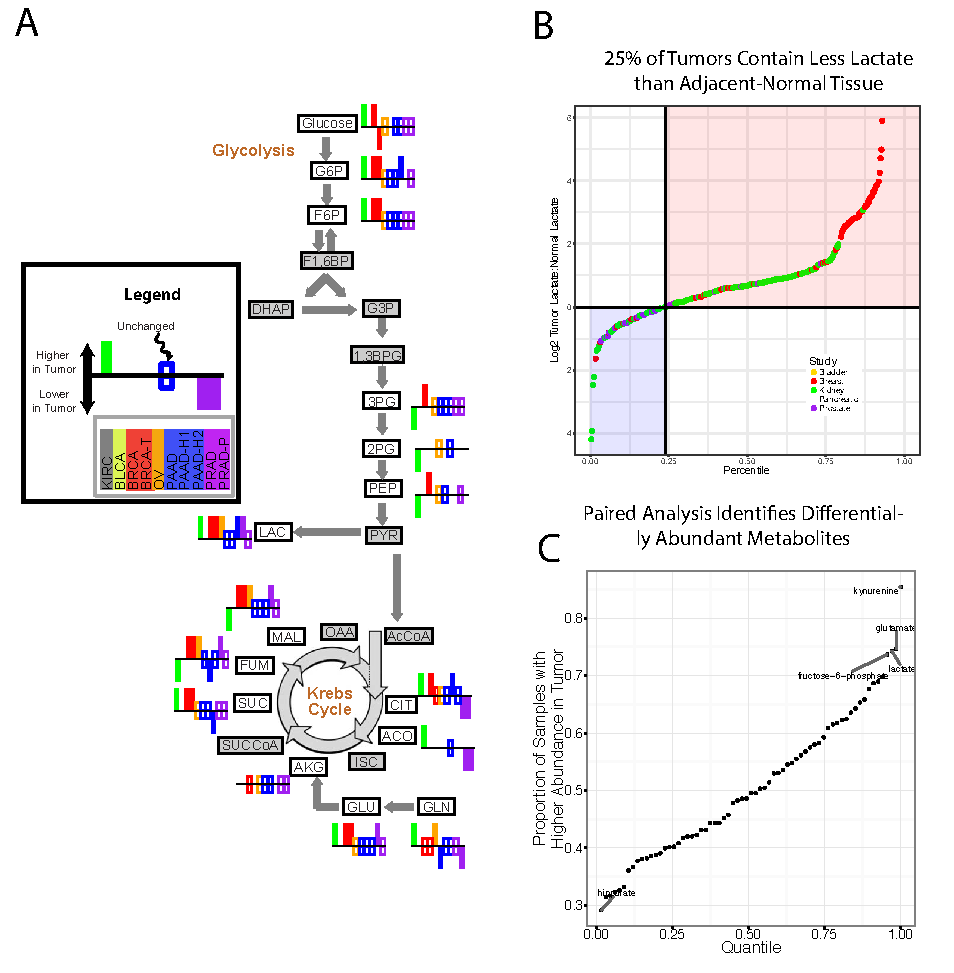
\includegraphics[scale = 0.5]{finalfigures/Figure5.pdf}
  \caption{\textbf{Metabolic correlation with tumor progression.} (A) and (B) Relatively few metabolites correlate with tumor stage and grade across multiple cancer types. (C) Kynurenine is significantly associated with tumor grade across three different cancer types (breast, gliomas, and  prostate cancers.}
     \label{fig:Fig5}
\end{figure}


\section{Discussion}

Tumors must bear the metabolic challenges faced by the tissue they arise, from the frequent osmotic stress inherent to the filtration performed by kidney cells to the xenobiotic stress endured by cells of the liver. Thus, it should come as no surprise that tumors  vary substantially in how their metabolic phenotype. In this study, we examined in detail the extent of this variation across nine cancer types. While we observed that some tumors (\textit{e.g.} of the prostate) appear to show comparatively minor metabolic alterations compared to other cancer types, we also found metabolic alterations common to the majority of cancer types (\textit{e.g.} the increase in abundance of lactate and kynurenine). 

Our approach to the assembly and alignment of several metabolomics studies relied on several computational pipelines which we expect to serve as a benchmark for future work. As described in detail earlier and in the Methods, the majority of data compiled here was reported in terms of (dimensinoaless) relative abundances, rather than absolute concentrations. To make data across studies comparable, we implemented a computational pipeline which assured, where possible, common standards for data imputation and standardization. We also implemented a bioinformatic pipeline to ``align'' metabolites identified by distinct metabolite identifiers, the code for which is included as a supplementary file (SI File XX). To compare results across studies, we relied heavily on non-parametric statistics, and used changes relative to normal tissue as the fundamental unit of comparison. 

\subsection{Caveats}
Sev
- Data quality: imputation, relative abundances
- Variability in sample prep


\subsection{Future Directions}
The results of our analysis are intended to be a starting point for future analysis integrating metabolic characterization of tumors into our understanding of tumor biology. Below we describe several promising challenges whose resolution would add to our understanding of the contribution of metabolism to oncogenesis.

Despite the growing number of studies characterizing metabolite abundances in human tissues, to our knowledge no methods exist for utilizing these data to infer what the rates at which metabolic reactions proceed, \textit{i.e.} metabolic flux. In contrast, beginning nearly a decade ago and associated with the proliferation of gene expression studies, many methods have been developed to integrate transcript abundances with genome-scale metabolic models to predict metabolic flux. While several algorithms have been proposed to jointly integrate metabolomics and transcriptomics data into GSMMs \cite{Reznik2013,ShlomiPaper}, it is clear that the transition to a model fully parametrized exclusively with metabolomics data is a major challenge. Most of the methods proposed to date asssume \textit{a priori} that the time-averaged change of metabolites either does not change, or is quantified directly. In contrast, metabolomics data on surgically resected tumors is limited to single time-point measurements. Furthermore, much of the effort invested in integrating metabolomics data into GSMMs has focused on prokaryotic organisms which lack intracellular compartments. Deconvolving the relative contributions of such compartments (\textit{e.g.} the mitochondria and the cytosol) to metabolite levels will likely be critical to making accurate flux predictions.

While our analysis in this paper has focused on non-parametric, univariate analysis of changes in metabolite levels between tumor and normal samples, other analyses which respect the limitations of the data (Figure \ref{fig:Fig2}) are possible. One example, which we have not explored, is a correlation analysis, akin to those proposed in several publications using gene expression and metabolomics data \cite{Reznik2015,etc}. It is possible that, by examination of changes in covariation patterns between metabolites between different subsets of samples (\textit{e.g.} tumor/normal, high stage/low stage tumors), the identification of putatively ``rewired'' metabolic pathways may be possible. By coupling such correlation analyses with GSMMs and the possible ways flux may be routed through them (so-called elementary flux modes \cite{EFMs}), progress may be made towards flux prediction.

Finally, given the proliferation of clinical genomic sequencing of cancer samples, it seems obvious to propose that connections be drawn with molecular subtypes and the metabolic landscape of tumors. Several prominent examples now exist of molecular alterations which manifest with, among other things, distinct metabolic phenotypes: \textit{KRAS} mutations in pancreatic adenocarcinomas induces macropinocytotic scavenging of extracellular nutrients, and hotspot \textit{IDH1} and \textit{IDH2} mutations produce 2-hydroxyglutarate, which induces DNA hypermethylation via inhibition of $\alpha$-ketoglutarate-dependent DNA demethylases. It is likely that other effects, perhaps more subtle but nevertheless impacting tumor viability, remain to be uncovered.

\section{Methods}

\subsection{Data Imputation and Standardization}
For data which was already imputed and standardized (including the BLCA, KIRC, BRCA, BRCATang, OV, PAADHussain1, PAADHussain2, PRADLODA studies), we used the data as reported by the original authors. For five studies (COAD,LGG,PAAD,PRAD,and STAD) for which no imputation was completed, we applied the following imputation and standardization procedure. For each metabolite, imputed values were set equal to the minimum measured abundance of that metabolite. Then, all measurements of the metabolite were median normalized. 

\subsection{Metabolite ID Mapping}
\textcolor{red}{Augustin please fill in}

\subsection{Differential Abundance Tests}
Differential abundance was calculated using the ratio of the average abundance of a metabolite in tumor tissue, to the average abundance of a metabolite in normal tissue. Statistical significance was assessed using non-paramatric Mann-Whitney U-tests.

\subsection{Pathway Differential Abundance Score}
The differential abundance score for a pathway was defined as

\begin{align*}
DA = \frac{I - D}{S}
\end{align*}

\noindent where $I$ is the number of measured metabolites in a pathway which increased in abundance relative to normal tissue, $D$ is the number which decreased, and $S$ is the total number of measured metabolites. A $DA$ score of 1 indicates that all metabolites increased in abundance, whereas a score of -1 indicates that all metabolites decreased in abundance, relative to normal tissue.

\subsection{Metabolomics Data Acquisition and Normalization}
Metabolomics data from prior, published work was obtained either through the corresponding journal, or by contacting the corresponding author. The data for all studies except COAD and STAD was reported in relative abundances, \textit{i.e.} the abundance of a metabolite $i$ in sample $j$ could only be compared to other values of metabolite $i$ in different samples from the same study. For COAD and STAD, absolute abundances were reported.

Because metabolomics data does not necessarily obey a known distribution, we applied minimal normalization techniques in order to make data minimally comparable across all studies. For each metabolite in a study, we calculated the median abundance, and normalized by this abundance. Given the unknown distribution of the data in our study, we used only non-parametric statistical tests (which are independent of data distribution) to assess changes in metabolite abundance.

\subsection{Association with Tumor Grade}
Different statistical tests were applied to identify correlation between metabolites and clinical features depending on the level of censoring in the data. If there is less than 20\% censoring within the tested set, the Jonckheere-Terpstra test (a non-parametric test which uses permutations to calculate the p-value) was used to examine ordered differences among classes . If there are more than 20\% but less than 80\% censored data, an exact log-rank trend test is used for interval (left) censored data. Both tests assume a metabolite should increase/decrease monotonically with stage/grade.  If there is more than 80\% censoring no test is used, and the metabolite is ignored. To summarize the tests across cohorts I use Fisher’s method to combine p-values. Note that resulting combined p-value is parametric. 

Since we are interested in finding associations of a common sign (\textit{e.g.} consistently positive correlation across multiple studies), one-sided p-values are calculated first, aggregate into a combined p-value using Fisher's method \cite{Whitlock2005}, and then transformed to two-sided combined p-value.

\bibliographystyle{plain}
\bibliography{panmet}

\beginsupplement
\newpage

\begin{table}
\centering
\begin{tabular}{ c c c c }
  \textbf{Study Name} & \textbf{Cancer Type} & Data Type & \textbf{Reference}  \\
  \hline
  BLCA & Bladder & Mass Spectrometry & \cite{Putluri2011} \\
  BRCA & Breast & Mass Spectrometry & \cite{Terunuma2014} \\
  BRCATang & Breast & Mass Spectrometry & \cite{Tang2014} \\
  COAD & Colorectal & NMR & \cite{Hirayama2009} \\
  KIRC & Clear-cell Renal Cell & Mass Spectrometry & \cite{Hakimi2015} \\
  LGG & Glioma & Mass Spectrometry & \cite{Chinnaiyan2012} \\
  OV & Ovarian & Mass Spectrometry & \cite{Fong2011} \\
  PAAD & Pancreas & Mass Spectrometry & \cite{Kamphorst2015} \\
  PAADHussain1 & Pancreas & Mass Spectrometry & \cite{Zhang2013} \\
  PAADHussain2 & Pancreas & Mass Spectrometry & \cite{Zhang2013} \\
  PRAD & Prostate & Mass Spectrometry & \cite{Sreekumar2009} \\
  PRADLODA & Prostate & Mass Spectrometry & \cite{Priolo2014} \\
  STAD & Stomach & NMR & \cite{Hirayama2009}
\end{tabular}
\caption{Summary of the published cancer tissue metabolomics studies examined in this work.}
\label{table:SITab_Studies}
\end{table}

\begin{figure}[ht!]
  \centering
     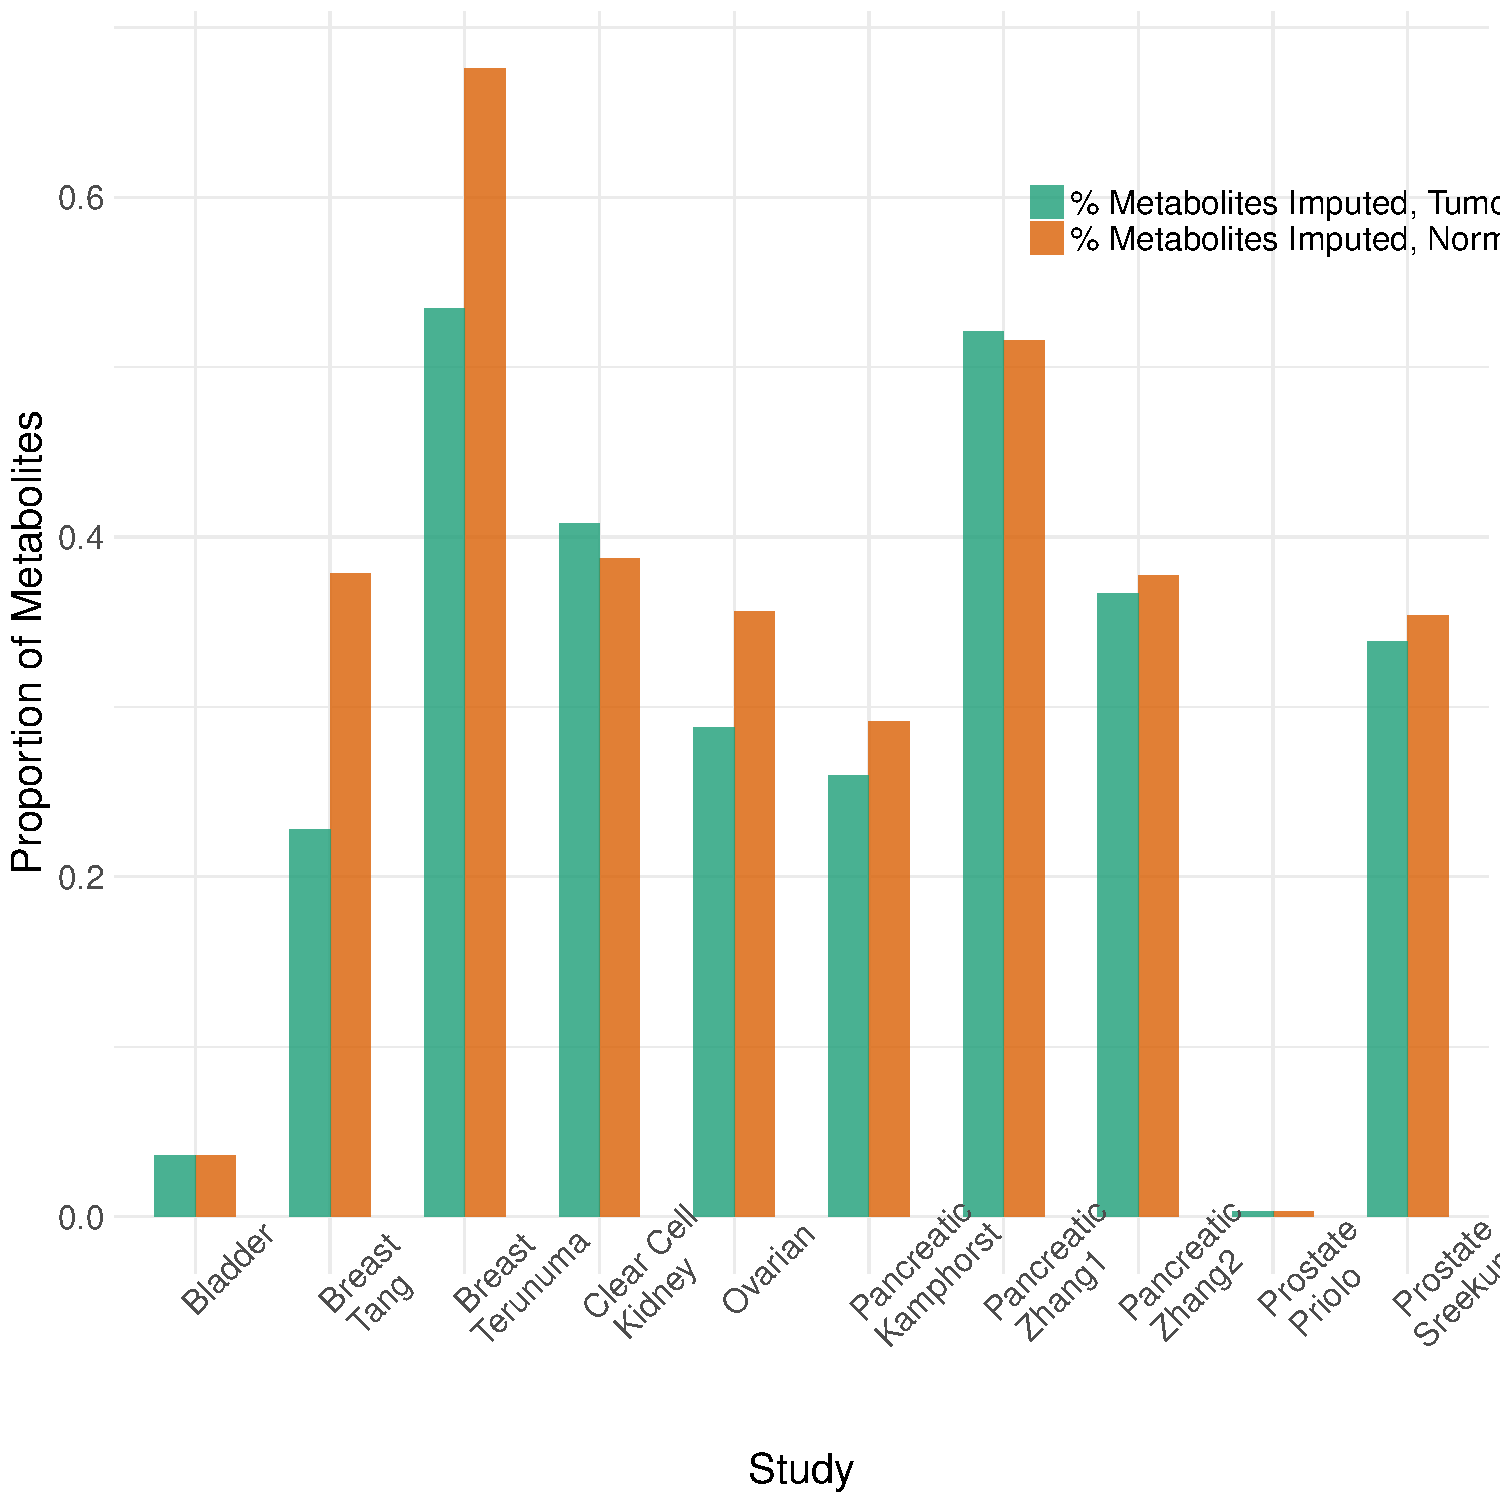
\includegraphics[scale = .6]{finalfigures/imput_barplot.pdf}
  \caption{For each study, we calculated the proportion of metabolites with greater than 20\% imputation in tumor samples. The calculation was repeated separately for normal samples. The two breast studies are exceptional because of the incongruent level of imputation between normal and tumor samples: far more metabolites are heavily imputed in normal breast samples, compared breast tumor samples. }
     \label{fig:SIFig_Imputation}
\end{figure}

\begin{figure}[ht!]
  \centering
     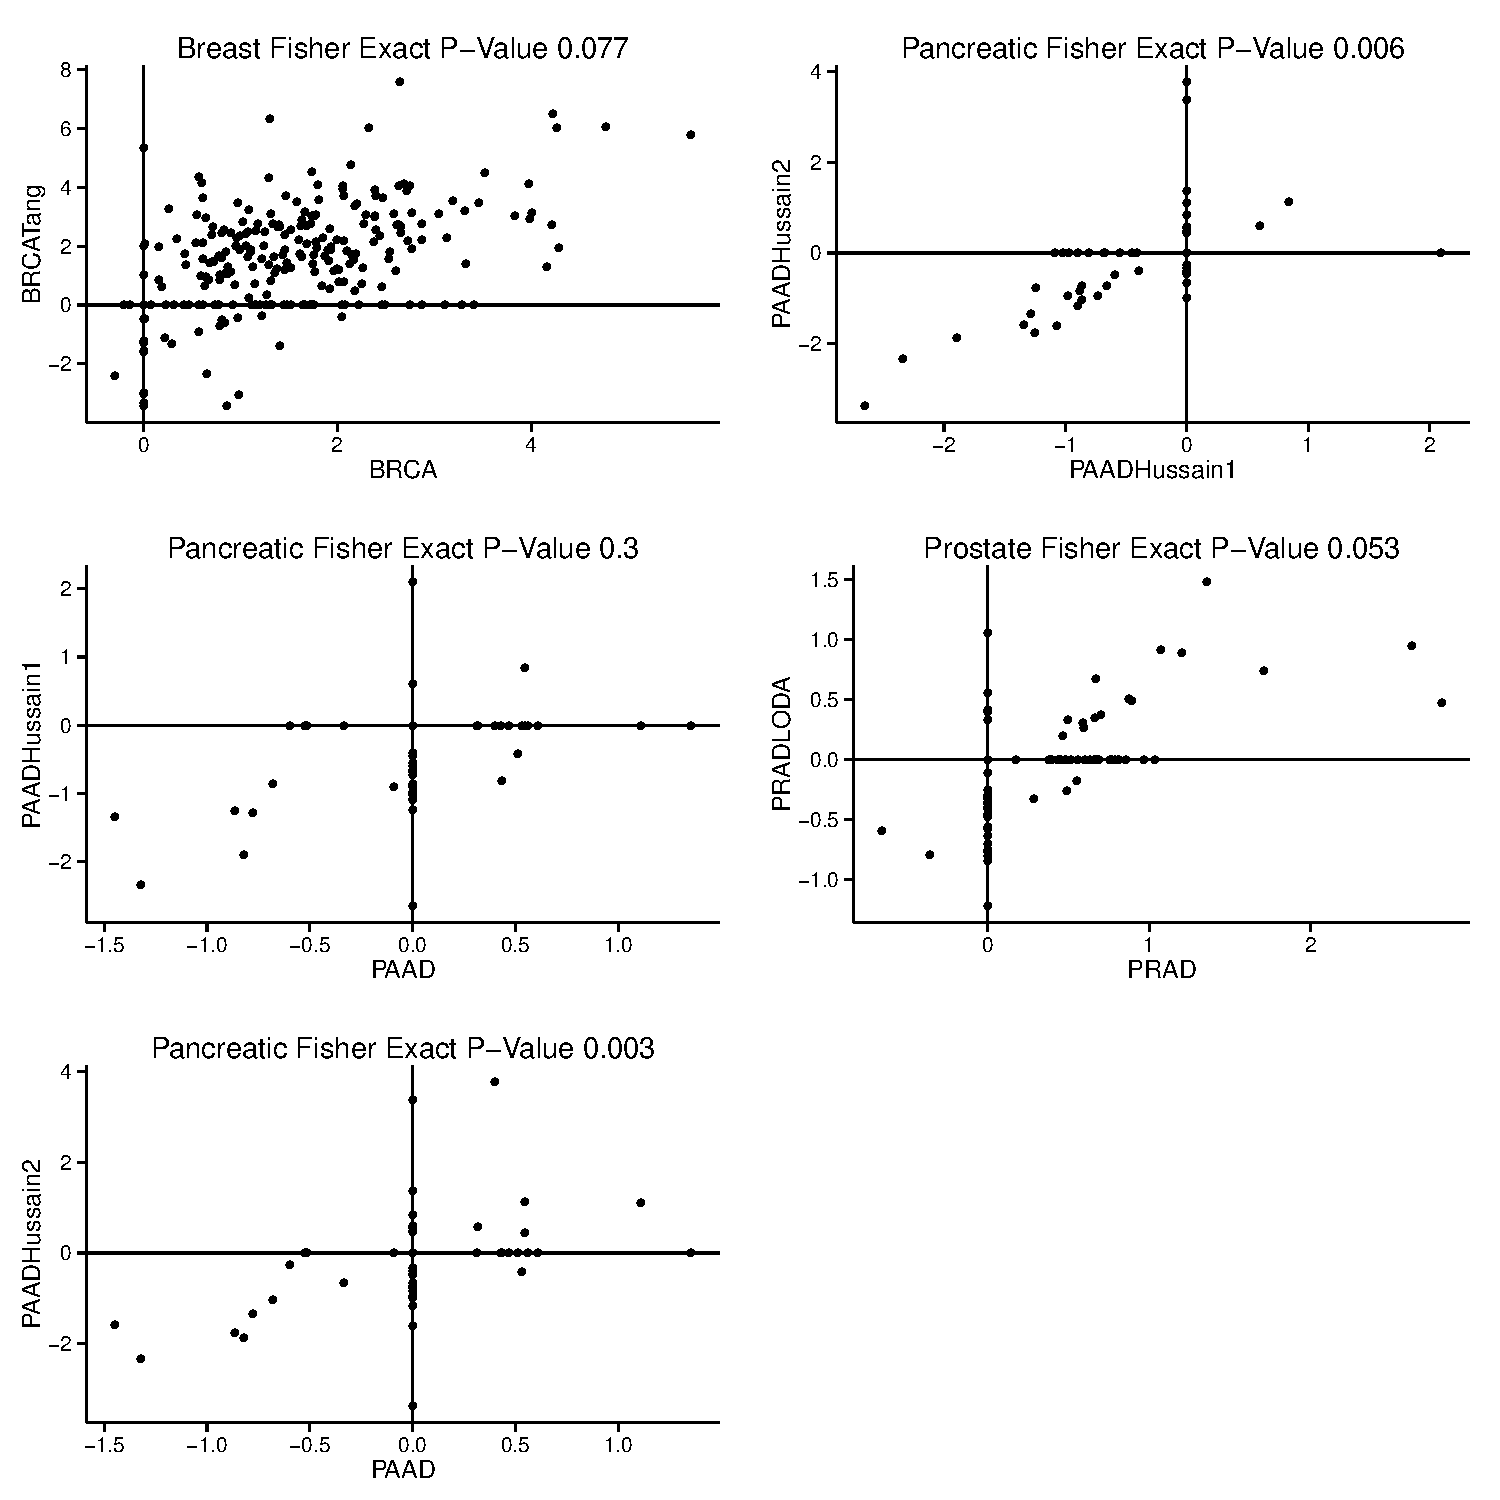
\includegraphics[scale = .6]{finalfigures/sametissue.pdf}
  \caption{Insert caption.}
     \label{fig:SIFig_SameTissue}
\end{figure}

\begin{figure}[ht!]
  \centering
     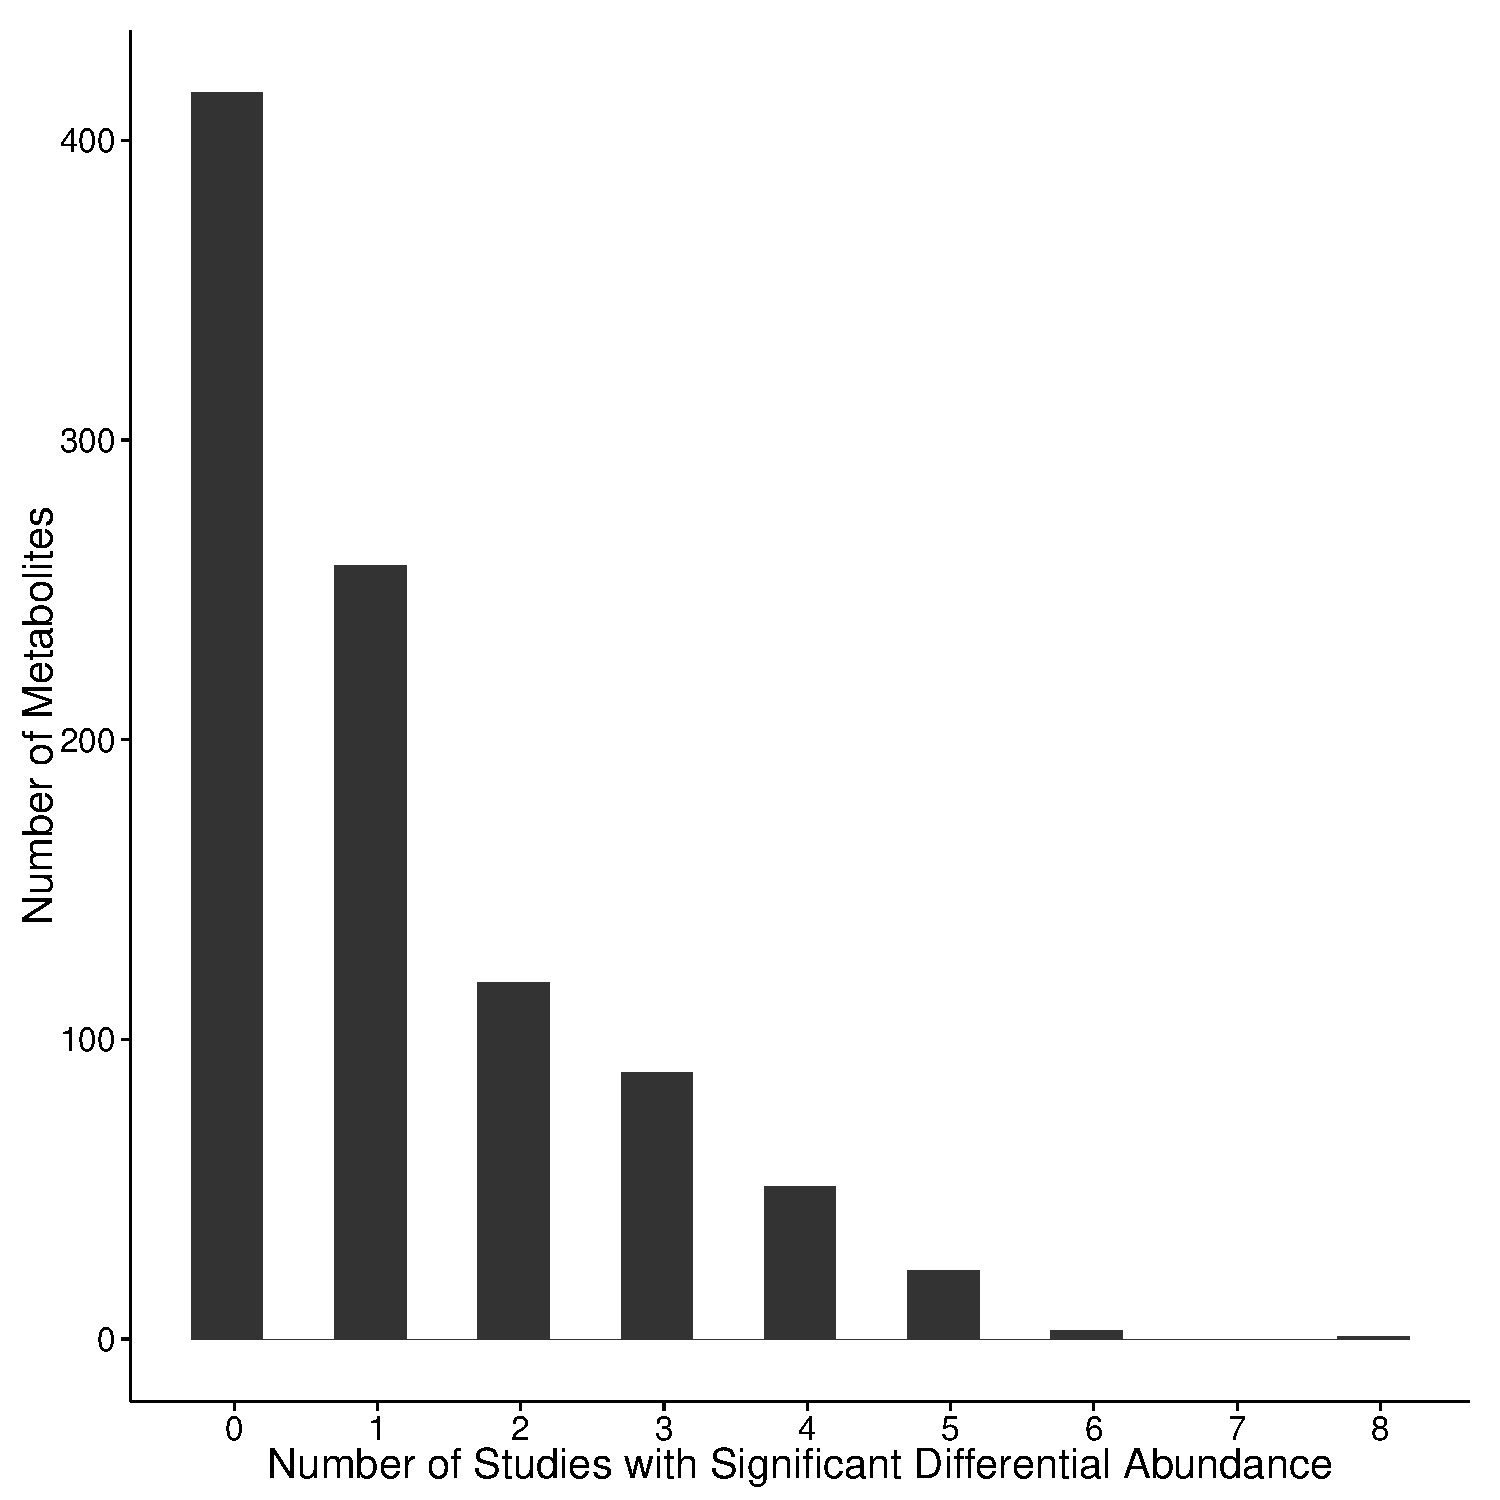
\includegraphics[scale = .6]{finalfigures/Histogram_NumDiffAbundant.pdf}
  \caption{Insert caption.}
     \label{fig:SIFig_HistogramDiffAbundance}
\end{figure}
 

\begin{figure}[ht!]
  \centering
     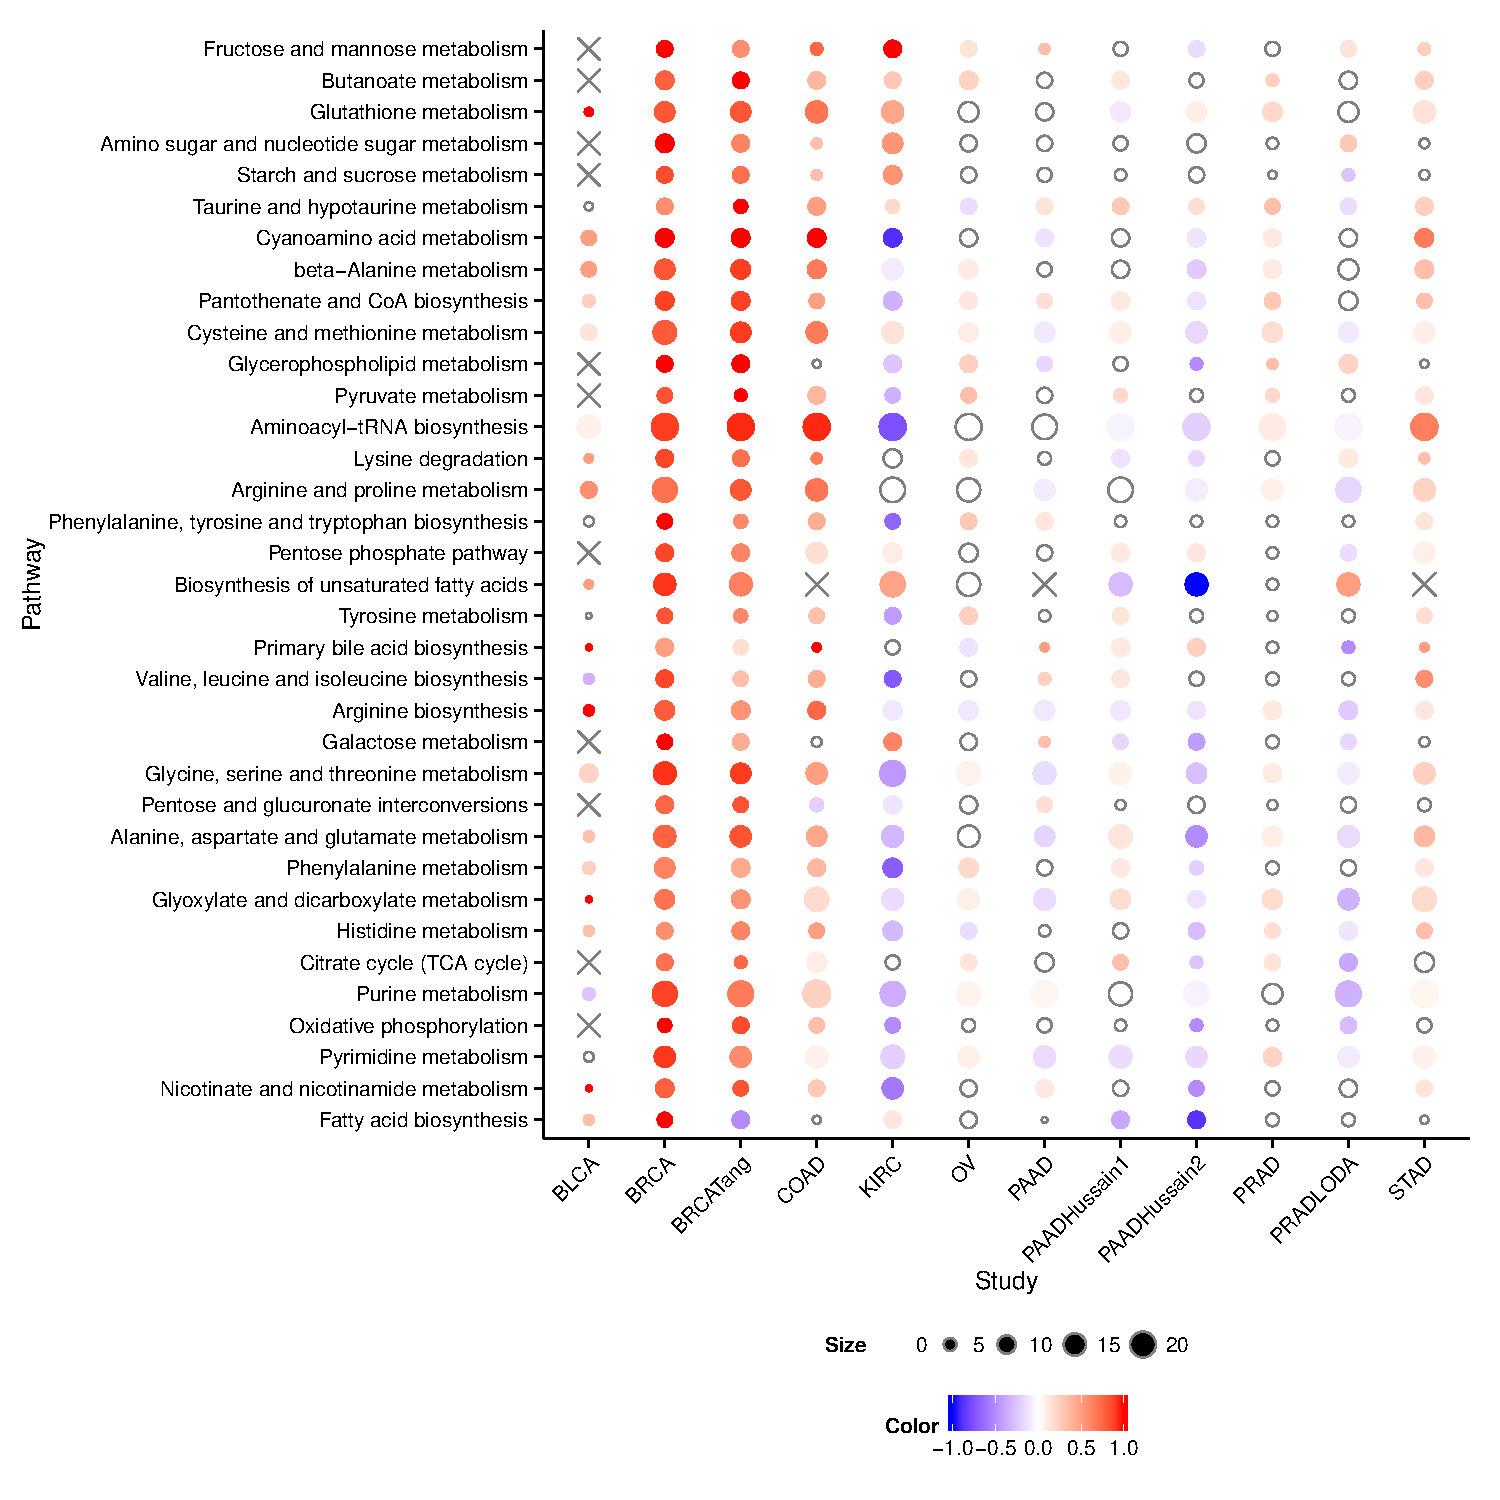
\includegraphics[scale = .6]{finalfigures/pathway_heatmap.pdf}
  \caption{Insert caption.}
     \label{fig:SIFig_PathwayHeatmap}
\end{figure}

\begin{figure}[ht!]
  \centering
     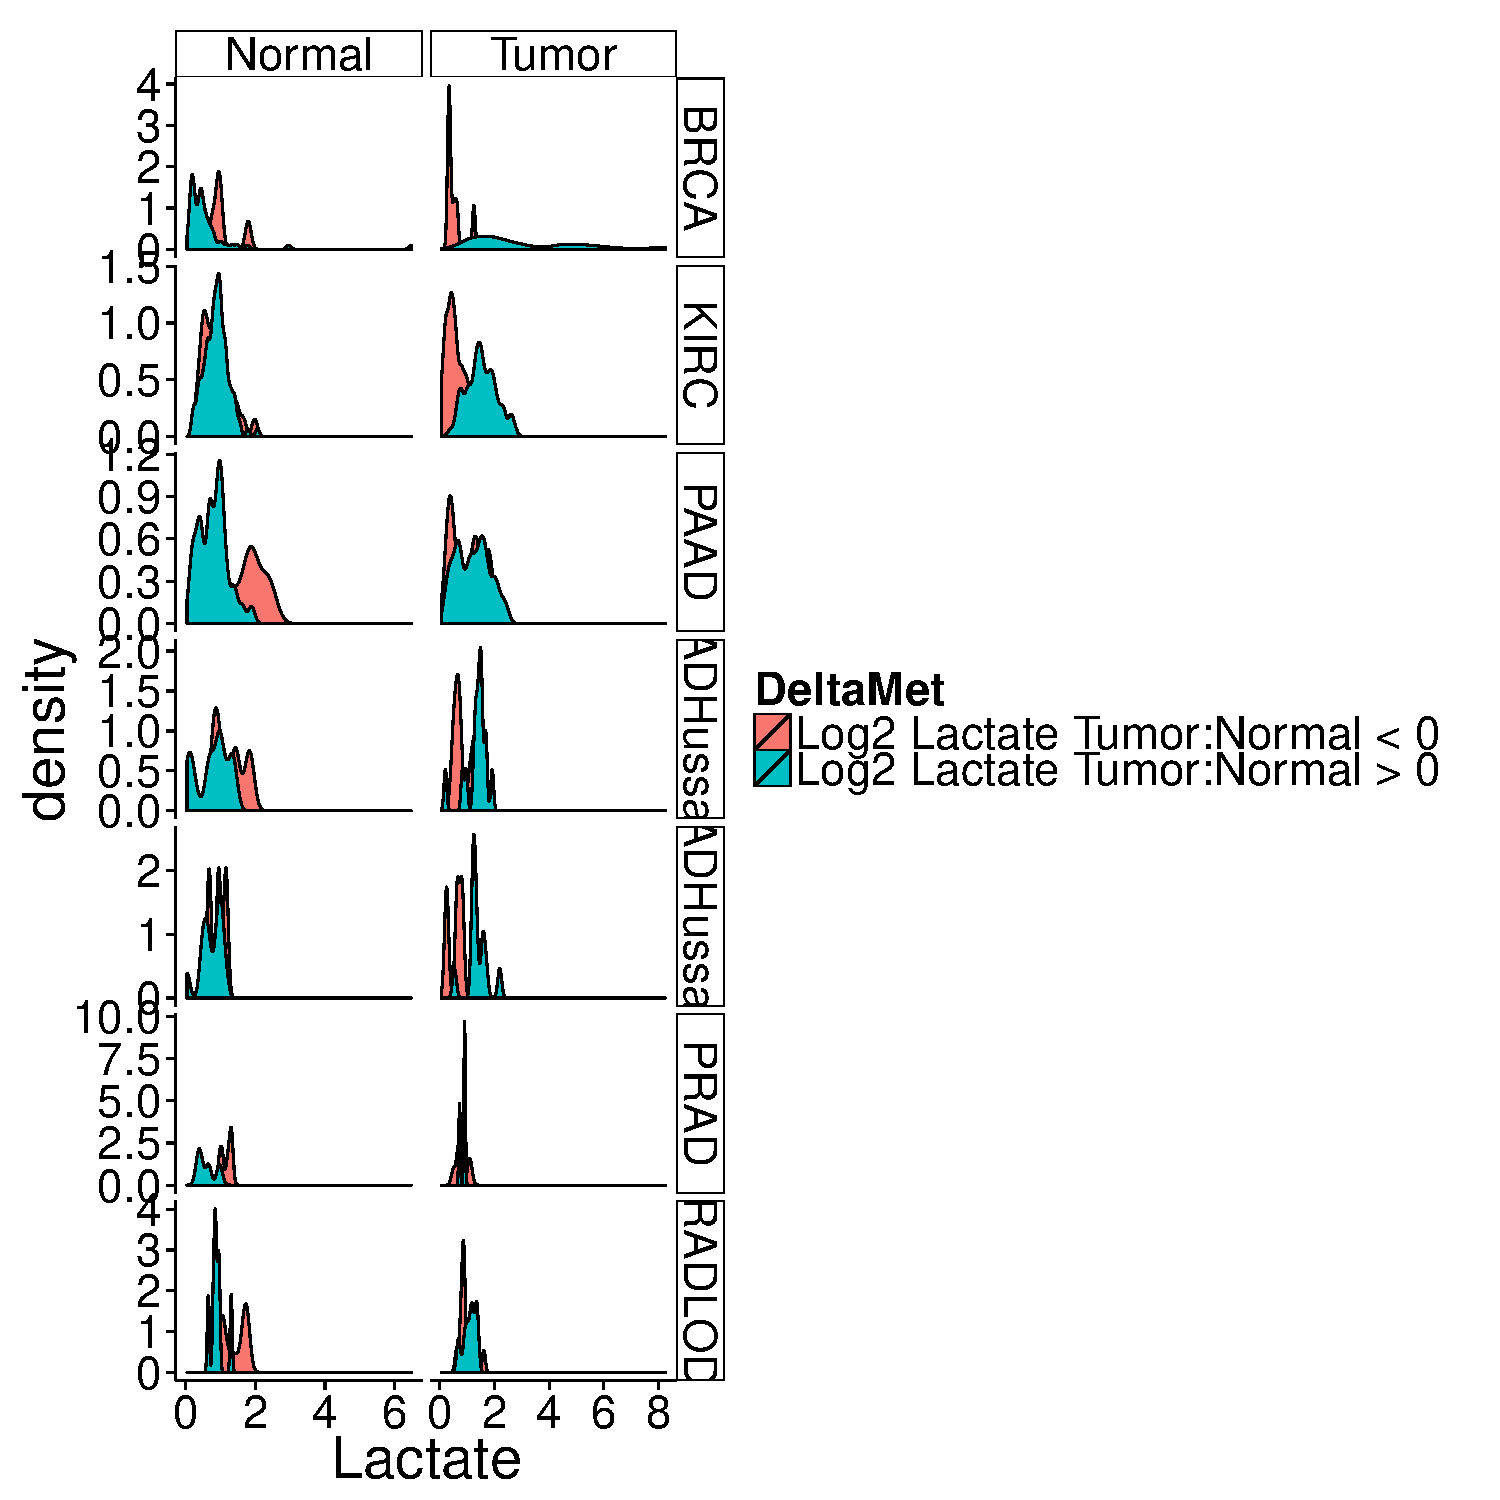
\includegraphics[scale = .6]{finalfigures/warburg_source.pdf}
  \caption{Insert caption.}
     \label{fig:SIFig_WarburgSource}
\end{figure}

\begin{figure}[ht!]
  \centering
     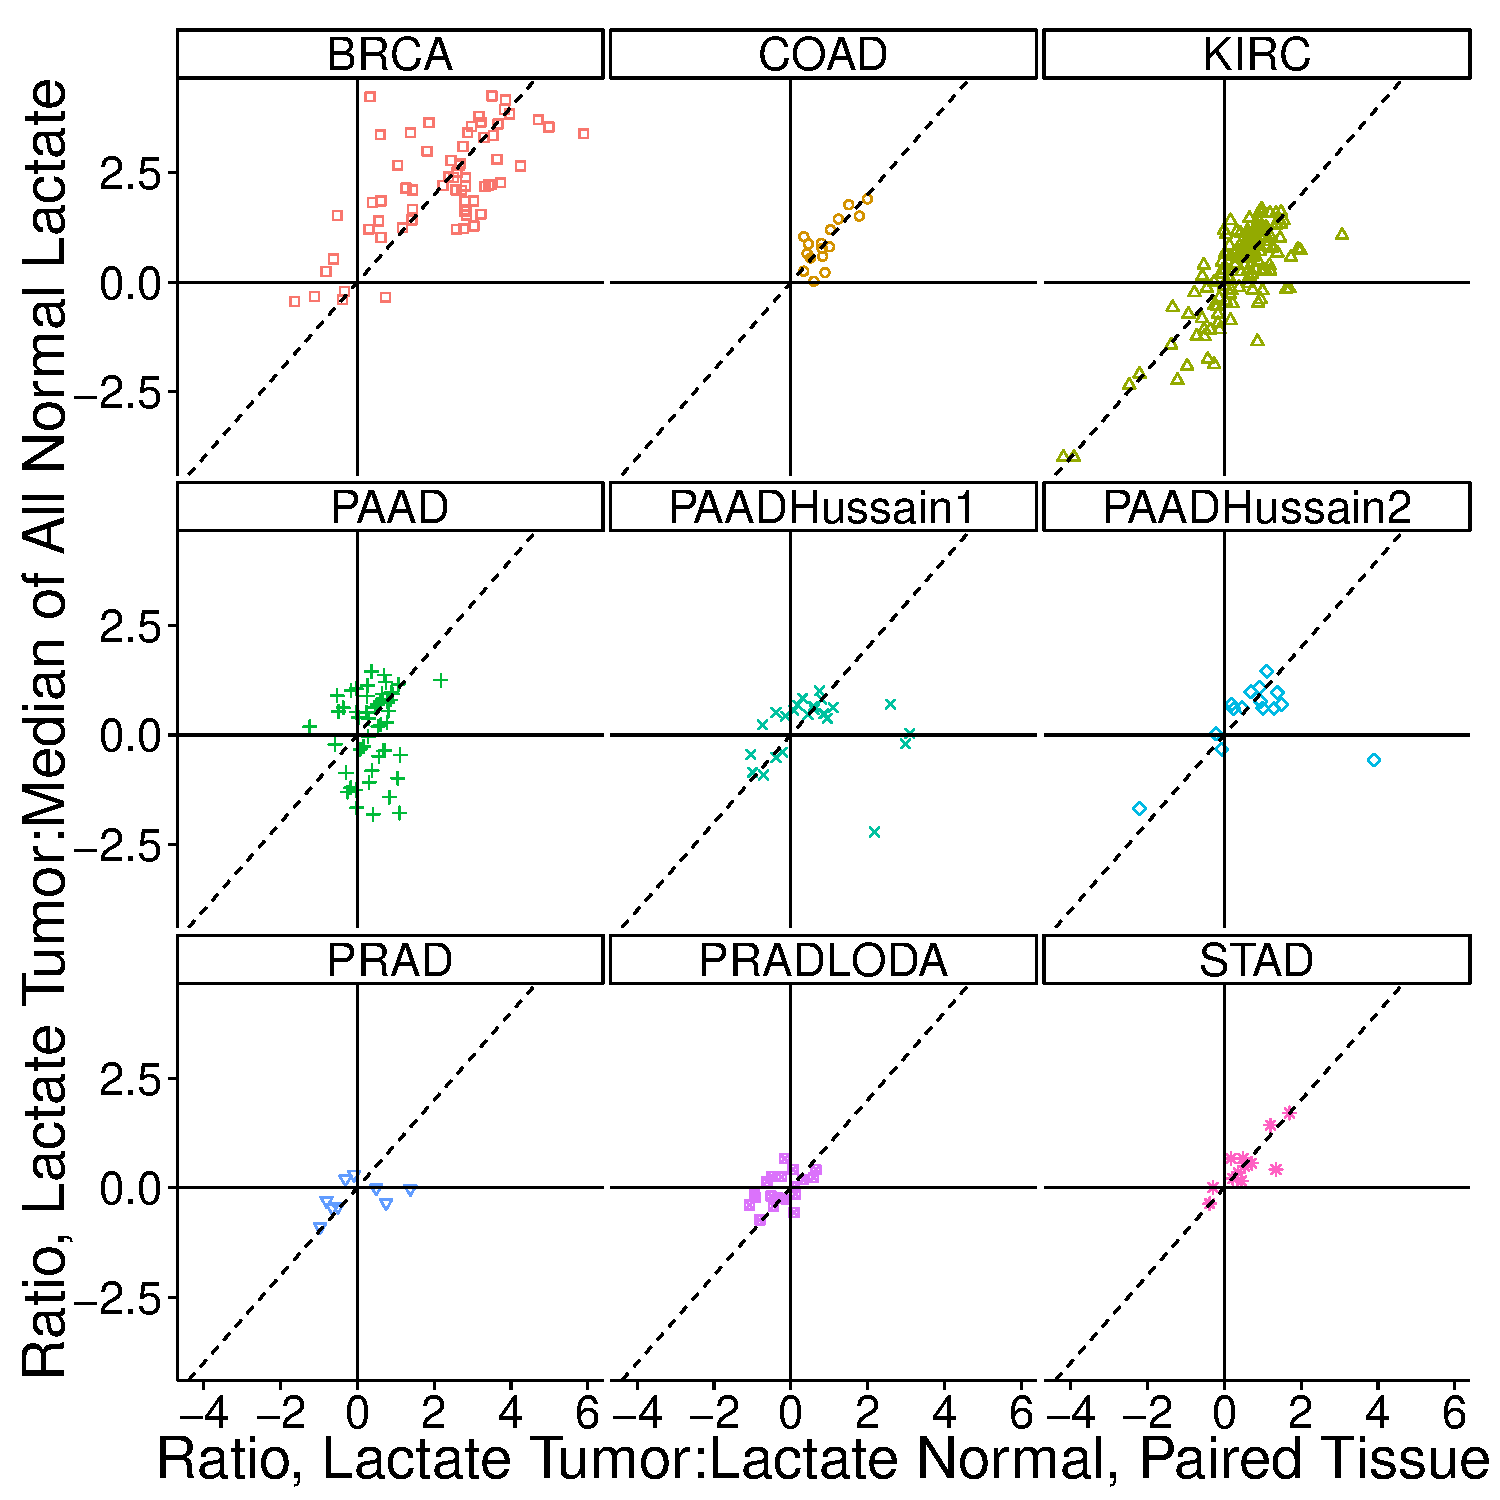
\includegraphics[scale = .6]{finalfigures/warburg_scatter.pdf}
  \caption{Insert caption.}
     \label{fig:SIFig_WarburgScatter}
\end{figure}

 
\end{document}
